\chapter{Weight Reparametrization}

\begin{abstract}
    abstract of this part
\end{abstract}

\section{Introduction And Related Work}

The introduction of neural networks has revolutionised the field of machine
learning, leading to breakthroughs in various areas such as image and speech
recognition, natural language processing, and game playing. However, the size of
neural networks has steadily increased in recent years, largely thanks to the
availability of powerful \ac{GPUs}. They have made it possible to train larger
and more complex models. However, as the size of neural networks has grown, so
have the computational and memory requirements to train and deploy them. The
evolution of neural network architectures can be traced back to the Rosenblatt
Perceptron \cite{rosenblatt1958perceptron}, a single-layer feedforward network
with only one neuron. Over time, neural network architectures became more
complex and began to include multiple layers, known as multilayer perceptron, or
fully connected networks. Then, with the introduction of \ac{CNNs}, neural
network architectures for image recognition have grown even larger.
Convolutional neural networks use convolutional layers to automatically and
adaptively learn spatial hierarchies of features from input images. This allows
\ac{CNNs} to effectively learn and classify images with high accuracy. Some of
the most notable \ac{CNN} architectures include AlexNet
\cite{DBLP:conf/nips/KrizhevskySH12}, which was developed in 2012 and has 60
million parameters. The VGG networks \cite{DBLP:journals/corr/SimonyanZ14a},
developed in 2014, are ranging from 132 to 143 million parameters. Inception
\cite{DBLP:conf/cvpr/SzegedyLJSRAEVR15}, developed in 2014, had 27 million
parameters in its third version. And the ResNet networks
\cite{DBLP:conf/cvpr/HeZRS16}, developed in 2015, are ranging from 11 to 60
million parameters. \\


The need for neural networks in embedded applications has grown in recent years,
with examples such as object detection in self-driving cars, image and speech
recognition in mobile devices, and natural language processing in smart
speakers. These applications require real-time processing and low power
consumption, which are impossible with large neural networks. Pruning techniques
can reduce the size of neural networks, making them more suitable for deployment
on embedded devices while still maintaining or even improving their performance.
Methods such as structured and unstructured weight pruning can reduce the number
of parameters and FLOPS, consequently reducing the network's size, memory and
power consumption.\\


Pruning is an excellent way to obtain lightweight neural networks because it
reduces the number of parameters in a pre-trained network without the need to
design a new architecture from the ground up. Instead of starting from scratch,
pruning techniques can be applied to existing architectures, which have been
trained and tested on large-scale datasets. It aims at reducing the number of
parameters in a network by removing redundant or unnecessary weights. Pruning
methods can be split into two major categories: unstructured weight pruning,
where individual weights of the network are removed based on their importance.
And structured pruning, where entire columns, rows, channels, filters or even
subnetworks are removed. \\


The first methods to prune shallow networks were proposed in the late 1980s.
Techniques from that area include removing the smallest connection
\cite{janowsky1989pruning}, introducing a weight scaling factor and the study of
its impact on the loss function \cite{DBLP:conf/nips/MozerS88} or the study of
the sensitivity of the weights based on the gradients
\cite{DBLP:journals/tnn/Karnin90}. Most influential papers of the early pruning
days are Optimal Brain Damage \cite{DBLP:conf/nips/CunDS89} and Optimal Brain
Surgeon
\cite{DBLP:conf/nips/HassibiS92,DBLP:conf/nips/HassibiSW93,DBLP:conf/icnn/HassibiSW93}.
The former work focuses on pruning weights based on their impact on the loss,
approximated by its Taylor series, which requires the computation of the hessian
matrix of the loss. However, computing the hessian matrix is Intractable in
practice due to the large number of parameters in the neural networks.
Therefore, the authors introduced a few simplifying assumptions, most notably
the diagonal assumption for the hessian matrix: loss perturbations following
weight pruning are assumed to be weight independent. \\


More recently, pruning regained traction with the work of Han et al.
\cite{DBLP:conf/nips/HanPTD15}.  The authors introduced a three-step pruning
method where first, the weights are tuned. Then all the weights whose absolute
value is below a certain threshold are removed. Finally, the remaining weights
are finetuned. \\


Following this work, research efforts stirred toward structured pruning.
Structured pruning removes groups of weights. The substructure of this group can
be a simple row or column in a filter, a channel of a filter, the filter itself
or even entire subnetworks. Structured pruning is not sparsifying weight
tensors, but rather reshaping the network to remove unnecessary parts of it that
are costly to evaluate and do not bring much performance improvement regarding
the considered task. Since the remaining weight tensors are not sparse, speedups
can be achieved with conventional libraries and hardware. In this context, Anwar
et al. \cite{anwar2017structured} proposed a pruning technique on various levels
(channels, kernels and intra-kernel levels) while Li et al.
\cite{DBLP:conf/iclr/0022KDSG17} proposed a pruning method at a larger (filter)
level. Network slimming \cite{DBLP:conf/iccv/LiuLSHYZ17} is a streamlined
approach that aims at pruning the most useless channels in the layers preceding
\ac{batch norm} \cite{DBLP:conf/icml/IoffeS15}. It induces sparsity with
$\ell_1$ penalization of the \ac{batch norm} scaling factors, each one
associated with a channel. Then channels are removed based on the relative
importance of their associated scaling factor, up to a predefined sparsity
ratio. More recent work proposed an automatic policy for pruning, such as
\ac{amc} \cite{DBLP:conf/eccv/HeLLWLH18} which relies on reinforcement learning
with two interacting agents; the first one iterates over the layers of the
architecture and defines a targeted sparsity, and the second agent implements
the targeted sparsity using channel pruning. The \ac{amc} algorithm is either
constrained by accuracy or efficiency, depending on the reward assigned to the
agents.  Going further with the concept of automatic pruning and architecture
search, Ramakrishnan et al. \cite{DBLP:conf/crv/RamakrishnanSN20} adapt $\ell_1$
penalization from \cite{DBLP:conf/iccv/LiuLSHYZ17} to model the relative
importance of layers, groups of layers or network parts that can be removed.
Following the same line, \cite{DBLP:conf/icml/KangH20} proposed a channel
pruning method based on batch normalization parameters. The authors introduce
masks which model the likelihood of feature maps being inhibited by the ReLU
activation function and thereby not contributing to the evaluation of the
underlying network. These masks are obtained by binarizing the cumulative
density function of the gaussian distribution parameterised by the scaling and
the shift of the BN layer. Masks and BN parameters are updated “end-to-end” with
a gradient estimated using the Gumble Softmax trick
\cite{DBLP:conf/iclr/JangGP17}. Authors claim that a high accuracy is maintained
after pruning and without fine-tuning. \\



Although convenient to implement in practice, structured pruning imposes a
strong topological prior by removing whole chunks in the primary network and
achieves a lower sparsity rate compared to unstructured pruning. On the other
hand, unstructured weight pruning focuses on removing independent weights from
the global structure. As a result, this method is much more flexible and leads
to high sparsity rates and compression ratios. Han et al.
\cite{DBLP:conf/nips/HanPTD15} introduced a simple yet effective three-step
algorithm for unstructured weight pruning: a first standard training step to
identify the most important connections, a magnitude pruning step to remove the
smallest weight and a final finetuning step to compensate for the loss of
accuracy. \cite{DBLP:journals/corr/HanMD15} used the same technique in
combination with quantization and Huffman coding, achieving a compression ratio
of up to 49x for a VGG16 network. Other methods do not rely on weight magnitude
such as \cite{DBLP:conf/iclr/LouizosWK18}, which uses non-negative stochastic
gates as a surrogate L0 norm and penalise non-zero weights during training.
Variational Dropout \cite{DBLP:conf/icml/MolchanovAV17} introduces a
multiplicative gaussian noise as an alternative to binary dropout
\cite{DBLP:journals/corr/abs-1207-0580,DBLP:journals/jmlr/SrivastavaHKSS14} with
an unbound dropout rate. Magnitude pruning regains significant attention after
the publication of the Lottery Ticket Hypothesis
\cite{DBLP:conf/iclr/FrankleC19}ttery Tickets, whose training with initial
weights taken from the large networks yields comparably accurate classifiers. To
extract the lottery ticket, it is necessary to train the large network up to
convergence, apply magnitude pruning and restore the original values of the
unpruned weights. This Lottery Ticket can then be trained to match the level of
performances of the large network, with at most the same number of epochs
needed. Although remarkable, this result is hardly applicable in practice since
it requires multiple computationally intensive training steps.\\


These structured or unstructured methods propose different saliency indicators
and pruning criteria that aim at identifying and removing redundant or
unnecessary weights or groups of weights in order to remove them. Removing
weights introduces a loss of functional performance - depending on the task
considered - that needs to be compensated for (with the exception of
\cite{DBLP:conf/icml/KangH20}). This is achieved through finetuning the sparse
or lightened networks obtained after applying the pruning criterion. Finetuning
is a computationally intensive task and requires additional training time.
Moreover, the amount of weights pruned is enforced after the initial training,
meaning that the final target size or weight budget is never considered in the
optimization procedure. Hence the need for a finetuning step. \\


In order to address the aforementioned issues, we introduce a novel
reparametrization that learns not only the weights of a surrogate lightweight
network but also its topology. This reparametrization acts as a regulariser that
models the tensor of the parameters of the surrogate network as the Hadamard
product of a weight tensor and an implicit mask. The latter makes it possible to
implement unstructured pruning constrained with a budget loss that precisely
controls the number of nonzero connections in the resulting network. Experiments
conducted on the CIFAR10 and the TinyImageNet classification tasks, using
standard primary architectures (namely Conv4, VGG19 and ResNet18), show the
ability of our method to train effective surrogate pruned networks without any
fine-tuning.

\section{Pruning With Weight Reparametrization And Budget Loss}

Consider the general case of a a multi-layer neural network, denoted as a
function $f$ of two variables: $\theta$ and $X$. $f$ can be seen as the topology
of the network: a computation graph whose edge values are given by $\theta$.
Indeed, $\theta$ is the set of weights of the network, so that $\theta =
\{\mathbf{w}_1, \mathbf{w}_2, \ldots, \mathbf{w}_L\}$, where $L$ is the number
of layer of the network. $X$ is the input taken by the network. The input $X$ is
an element of a dataset $\mathcal{D}=\{ \mathcal{X}, \mathcal{Y} \}$, where
$\mathcal{X}$ is the set of the input data, and $\mathcal{Y}$ is the set of the
corresponding labels. The elements of $\mathcal{X}$ and $\mathcal{Y}$ are real
valued tensors.

\begin{equation}
    % \centering
    \begingroup
  \setlength\arraycolsep{0pt}
  f \colon\begin{array}[t]{c >{{}}c<{{}} c}
             \mathbb{R}^{\dim (X)} & \to & \mathbb{R}^{\dim (y)} \\ 
             X & \mapsto & f(X, \theta) = \hat{y} 
          \end{array}
  \endgroup
\end{equation}

Evaluating the neural network $f(X_i, \theta)$ yields the output $\hat{y_i}$
which is the prediction of the network for the input $X_i$. The discrepancy
between the output of the neural network $\hat{y_i}$ and the ground truth $y_i
\in \mathcal{Y}$ is computed with a loss function $\mathcal{L}$.  This loss is
then minimized by updating the parameters $\theta$ of the network, thanks to the
backpropagation \cite{rumelhart1985learning,rumelhart1986learning} and gradient
descent methods.\\

The $L_0$ norm is perfectly suited for introducing sparsity in a network by, on
the one hand, acting as a sparsity-inducing regulariser for the weights, and on
the other hand, by indicating the number of non-zero weights in the network,
which is useful for computing the weight budget. \\

Our aim is to propose an end-to-end method that fits into the backpropagation
framework. Therefore, adding a $L_0$ regulariser and a $L_0$ based weight budget
is not possible since $L_0$ norm is not differentiable. Thus we propose our
differentiable reparametrization, which seeks to define a novel weight
expression related to magnitude pruning
\cite{DBLP:conf/nips/CunDS89,DBLP:conf/nips/HanPTD15}. This expression
corresponds to the Hadamard product involving a weight tensor and a function
applied entry-wise to the same tensor (as shown in
\cref{fig:chap1:comparison_reparam_vs_mag_pruning}). This function acts as a
mask that i) multiplies weights by soft-pruning factors which capture their
importance and ii) pushes less important weights to zero through a particular
budget added to the loss function $\mathcal{L}$. \\

\begin{figure}[h]
    \centerline{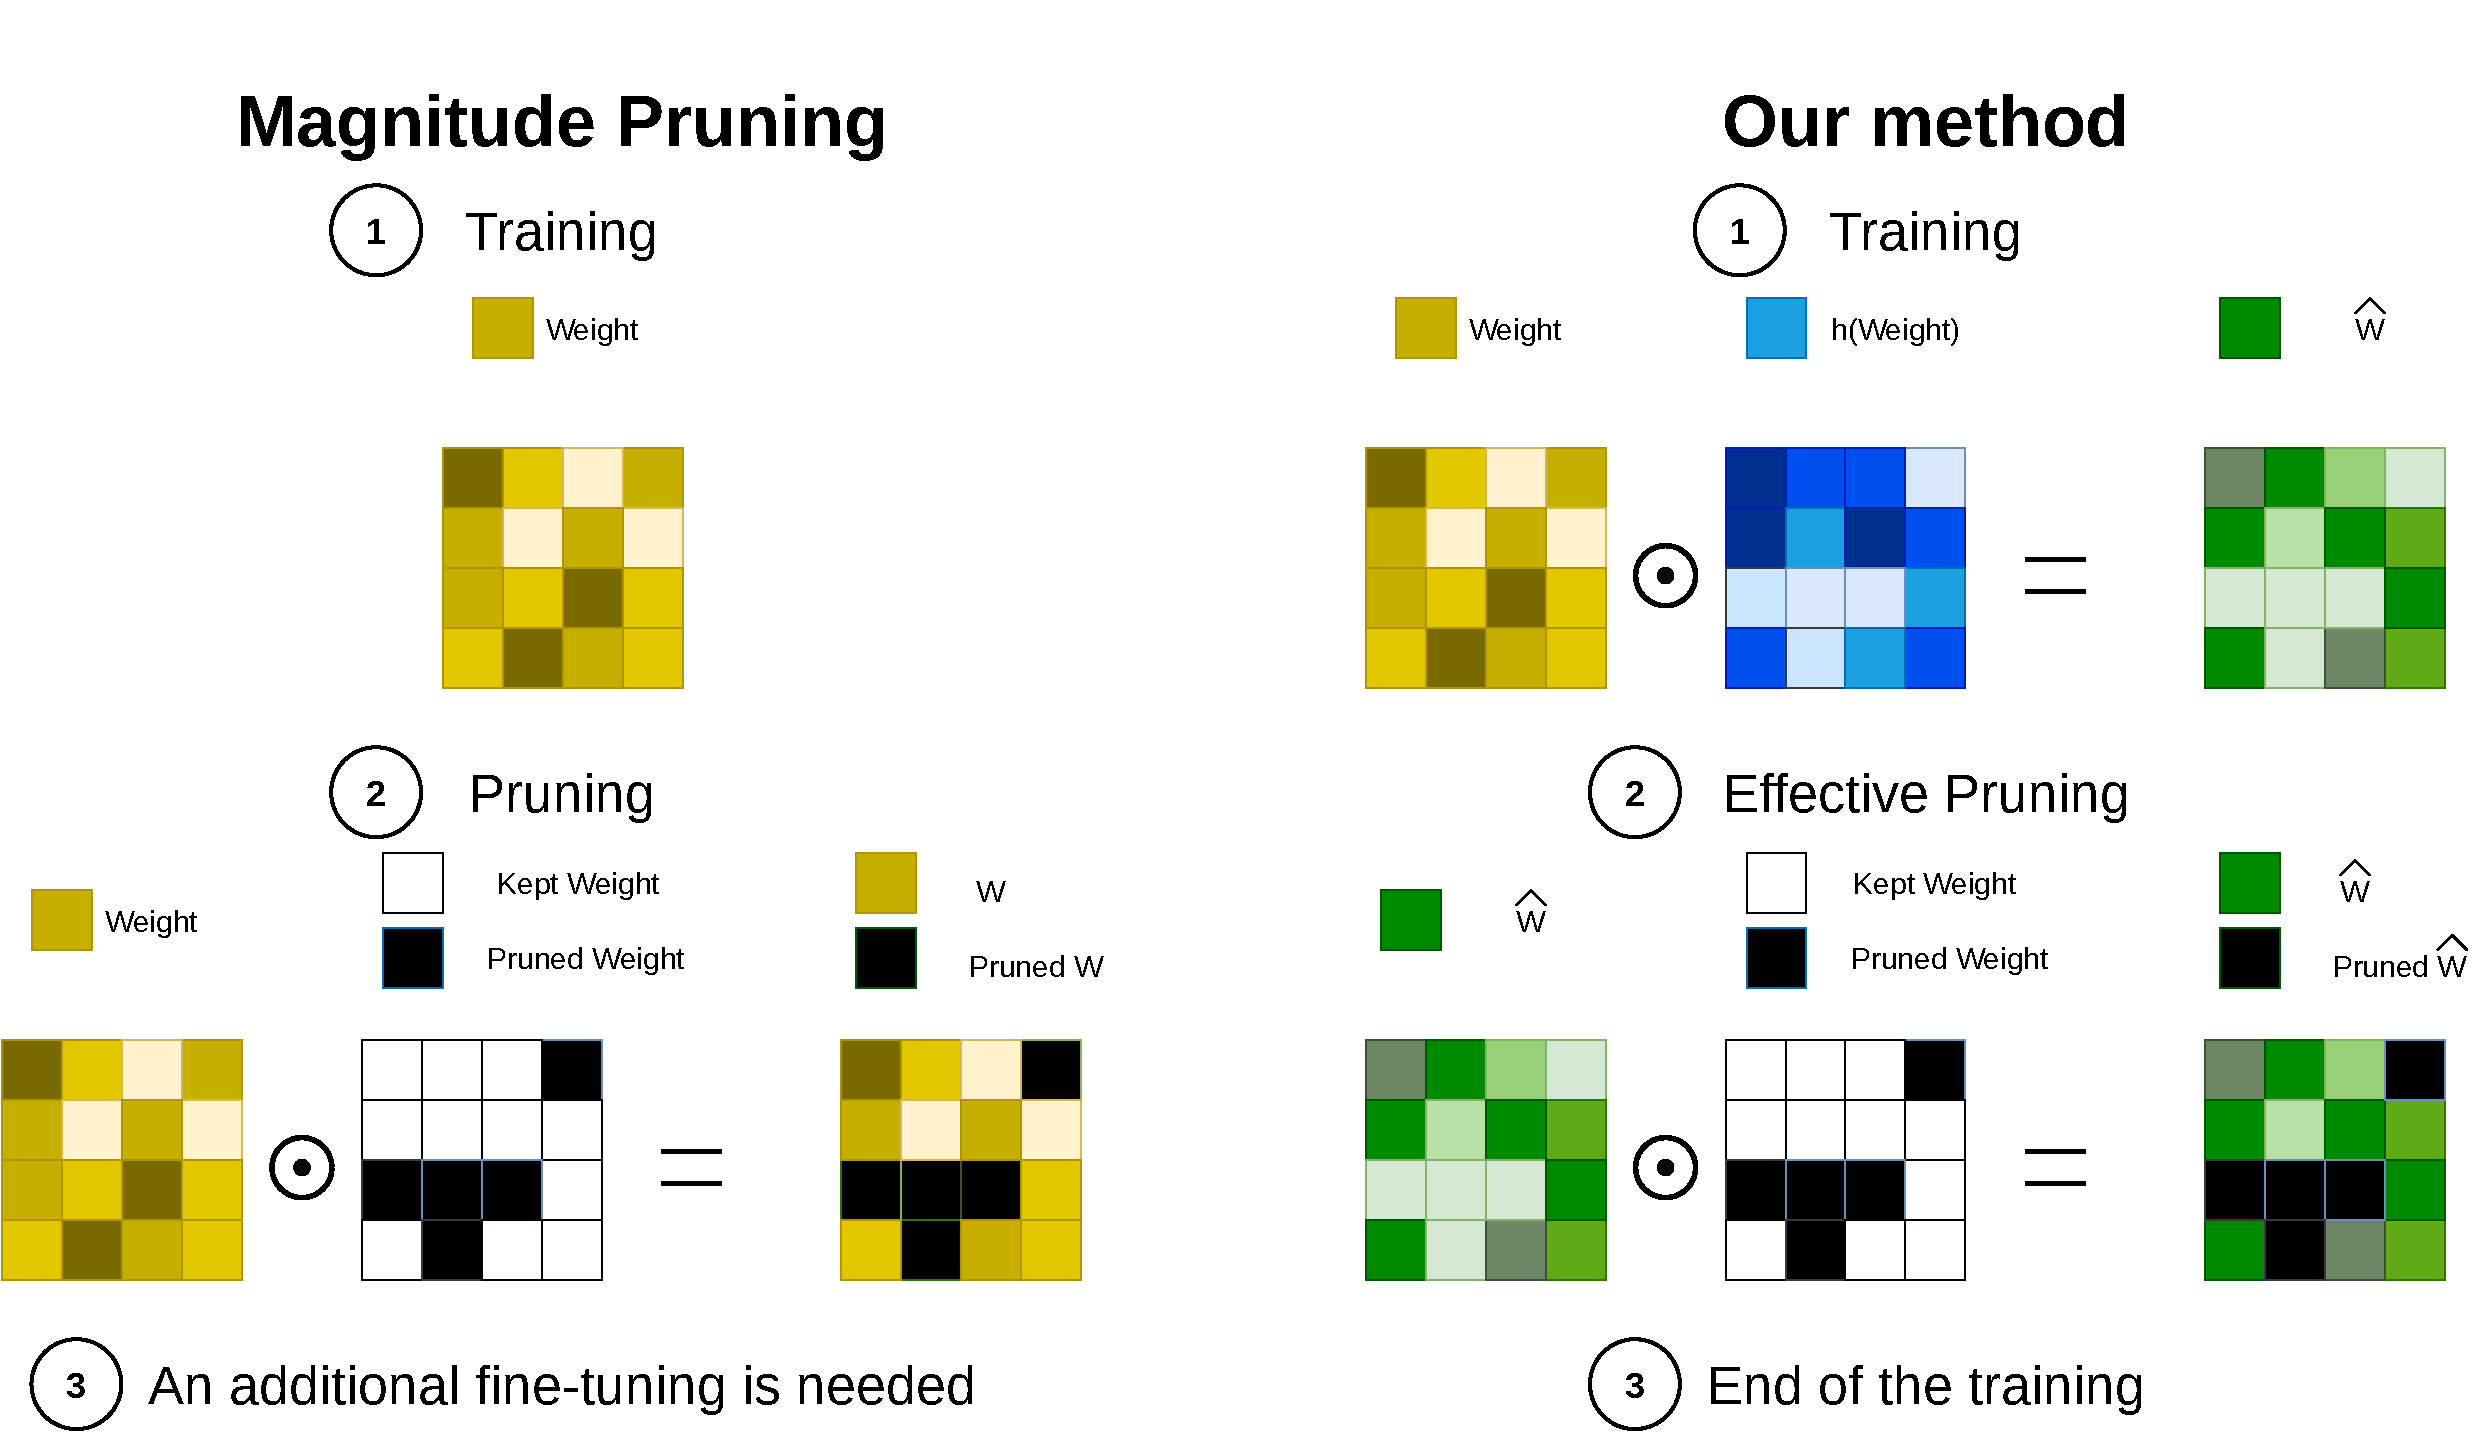
\includegraphics[width=12.5cm]{chapter_1/assets/comparison_reparam_vs_mag_pruning.pdf}}
  \caption{Comparison of our method and magnitude pruning. Magnitude pruning
  does not include any prior on the weights during the initial training phase
  and needs an additional fine-tuning procedure. Our method embeds a saliency
  heuristic based on the weight magnitude in the weight reparametrization and
  does not requires fine-tuning.}
  \label{fig:chap1:comparison_reparam_vs_mag_pruning}
\end{figure}


Our proposed framework allows for a joint optimization of the network weights
and topology. On the one hand, it prevents disconnections which may lead to
degenerate networks with an irrecoverable performance drop. On the other hand,
it allows reaching a targeted pruning budget in a more convenient way than $L_1$
regularization. Our reparametrization also helps minimizing the discrepancy
between the primary and the surrogate networks by maintaining competitive
performances without fine-tuning. Learning the surrogate network requires only
one step that achieves pruning as a part of network design. This step zeroes out
the targeted number of connections by constraining their reparametrized weights
to vanish.

\subsection{Weight Reparametrization}
\label{sec:chap1:weight_reparam}

We consider the priramy network $f$ as a combination of $L$ layers. The global
expression of $f$ can be recursively defined the application of the layer $\ell$
to the output of the layer $\ell-1$. Without a loss of generality, we omit the
bias for the sake of clarity. This expression is shown on
\cref{eqn:chap1:layer_eq_f}.
\begin{equation}
\label{eqn:chap1:layer_eq_f}
f(\mathbf{x}) = g_L \big(\mathbf{w}_L \cdot g_{L-1}(\mathbf{w}_{L-1} \cdot g_{L-2} \dots
\mathbf{w}_2 \cdot g_1(\mathbf{w}_1 \cdot \mathbf{x}))\big),
\end{equation}
\noindent with $g_\ell$ being a nonlinear activation associated to $\ell \in
\left\{ 1,\dots, L \right\}$ and $\left\{ \mathbf{w}_\ell \right\}_\ell$ a
weight tensor. Keeping the same topology but changing the values of the weight,
we now consider the surrogate network $\hat{f}$ with weights
$\{\hat{w}_\ell\}_\ell$. \Cref{eqn:chap1:layer_eq_f} now becomes
\cref{eqn:chap1:layer_eq_f_hat}. The activation function and the topology of $f$
and $\hat{f}$ are the same. Only the weights are changing.

\begin{equation}
\label{eqn:chap1:layer_eq_f_hat}
\hat{f}(\mathbf{x}) = g_L \big(\mathbf{\hat w}_L \cdot g_{L-1}(\mathbf{\hat w}_{L-1} \cdot g_{L-2}
\dots\mathbf{\hat w}_2 \cdot g_1(\mathbf{\hat w}_1 \cdot \mathbf{x}))\big).
\end{equation}

\noindent In the above \cref{eqn:chap1:layer_eq_f_hat}, $\mathbf{\hat w}_\ell$
is referred to as apparent weight. The apparent weight is a reparametrization of
$\mathbf{w}_\ell$, that includes a prior on its saliency. An apparent weight
$\mathbf{\hat w}_\ell$ of $\hat{f}$ is derived from the standard weight
$\mathbf{w}_\ell$ of $f$ by applying the following reparametrization: 
\begin{equation}
  \label{eqn:reparam}
  \mathbf{\hat w}_\ell = \mathbf{w}_\ell  \odot h_t(\mathbf{w}_\ell),
\end{equation}
\noindent with $h_t$ being the reparametrization function and $t$ its
temperature parameter. This reparametrization function enforces the prior that
smallest weights should be removed from the network and act as a surrogate $L_0$
norm for the budget loss (see \cref{sec:chap1:budget_loss}). In order to achieve
this objective, $h_t$ should exhibit four properties: \\

\begin{enumerate}
  \item $\forall x \in \mathds{R},~~ 0 \leq h_t(x) \leq 1 $
  \item $h_t(x) \in C^1 \text{ on } \mathds{R}$
  \item $h_t(x) = h_t(-x)$
  \item $\forall a,\varepsilon \in\mathds{R}^{+\ast},~ \exists ~t
  \in\mathds{R}^{+\ast} ~ | ~ h_t(x) \leq \varepsilon, x \in [-a,a]$
\end{enumerate}

\noindent\textbf{First Property - Constrained Image} \\
\begin{equation}
    \centering
    \forall x \in \mathds{R},~~ 0 \leq h_t(x) \leq 1
    \label{eqn:chap1:reparam_prop1}
\end{equation}
\\
There should not be any co-adaptation between the weights and its
reparametrization. Indeed, the reparametrization function should not act as a
scaling factor for the weight and scale it so that the apparent weight is larger
than the original weight. Finally, the apparent weight should have the same sign
as the original weight. That's why the image of $\mathbb{R}$ by $h_t$ should be
the segment $[0,1]$.\\

\noindent\textbf{Second Property - Differentiability} \\
\begin{equation}
    \centering
    h_t(x) \in C^1 \text{ on } \mathds{R}
    \label{eqn:chap1:reparam_prop2}
\end{equation}
\\
Our method should fit in the backpropagation method. Since the optimization will
be achieved by gradient descent, the reparametrization function should be
derivable to ensure that it has a computable gradient.\\

\noindent\textbf{Third Property - Symmetry} \\

\begin{equation}
    \centering
    h_t(x) = h_t(-x)
    \label{eqn:chap1:reparam_prop3}
\end{equation}
\\
The reparametrization function should not induce any bias toward the positive or
negative weights, so that only their magnitudes matter. It implies that the
reparametrization function should be symmetric with respect to the origin.\\


\noindent\textbf{Fourth Property - } \\

\begin{equation}
    \centering
    \forall a,\varepsilon \in\mathds{R}^{+\ast},~ \exists ~t
    \in\mathds{R}^{+\ast} ~ | ~ h_t(x) \leq \varepsilon, x \in [-a,a]
    \label{eqn:chap1:reparam_prop4}
\end{equation}
\\
The last property ensures the existence of a temperature parameter $t$, which
allows upper-bounding the response of $h_t$ on any interval for any arbitrary
$\varepsilon$. More formally, for any arbitrarily large $a$ and arbitrarily
small $\varepsilon$, it exists a temperature $t$ which guarantees that the
reparametrization of any $x$ is smaller than $\varepsilon$, provided that $x$ is
in the segment $[-a, a]$. Hence, $h_t$ acts as a stopband filter which
eliminates the smallest weights where the parameter $t$ controls the width of
that filter. \\



\begin{figure}
    \centering
    \subfloat[$h_{t}$ with $t=1$ and varying $n$]{
        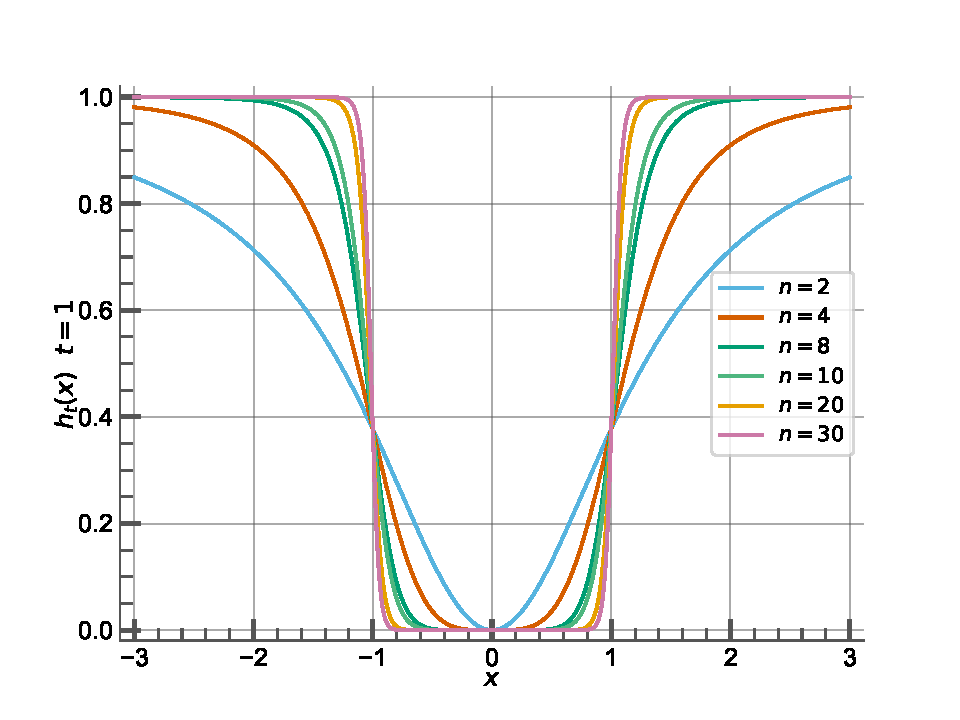
\includegraphics[height=0.36\linewidth]{chapter_1/assets/reparam_funct_varying_n.pdf}
        \label{fig:chap1:reparam_funct_varying_n}} \subfloat[$h_{t}$ with $n=2$
    and varying $t$]{
        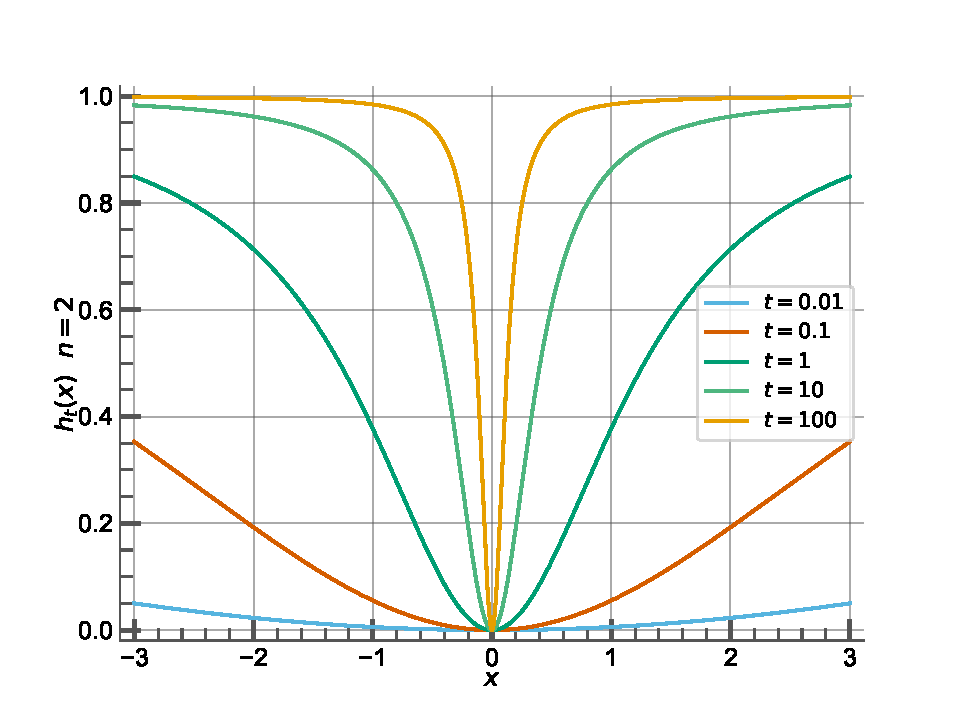
\includegraphics[height=0.36\linewidth]{chapter_1/assets/reparam_funct_varying_t.pdf}
        \label{fig:chap1:reparam_funct_varying_t}} \caption{\centering
    Reparametrization function $h_t$ with varying temperature parameter $t$ and
    power $n$. $t$ controls the width of the pit and $n$ controls the steepness
    of the slope.}
    \label{fig:stopband}
\end{figure}

Weight distribution varies greatly from one layer to another. In order to match
a specific budget (see \cref{sec:chap1:budget_loss}), the width of the stopband,
controlled by $t$, is tuned according to the weight distribution of each layer.
The manual setting of this parameter is difficult and cumbersome, so in
practice, $t$ is learned as a part of gradient descent on a layer-by-layer
basis.\\

% TODO: Ajouter amorce pour discussions sur l'initialisation de la température.
%the initial setting  $t_\text{init}$ of this temperature is shown in
%\cref{tbl:pruningperformances}.\\


Considering the aforementioned four properties of $h_t$, a simple choice of that
function is 
\begin{equation}
  \label{eqn:chap1:h_star_expression}
  h_t^*(x) = \exp\bigg\{{-\displaystyle\frac{1}{(tx)^n}}\bigg\}, ~ n\in 2\mathds{N},
\end{equation}
\noindent where $n$ controls the crispness of $h_t^*$. $n$ is not considered as
a parameter of $h_t$ (or $h_t^*$) since we use a fixed value for our
experiements, whereas $t$ is a learnt parameter and varies from one layer to
another. Although the function described in \cref{eqn:chap1:h_star_expression}
satisfies the four above properties, $h_t^*$ suffers from numerical instability
as it generates \ac{nan} outputs in most of the widely used deep learning
frameworks. Due to the way Backpropagation works, a single \ac{nan} in a weight
tensor makes the whole optimization process for the entire network no longer
possible. We consider instead a stabilized variant with a similar behavior, as
\cref{eqn:chap1:h_star_expression},  that still satisfies the four above
properties (see also \cref{fig:chap1:h_stable_vs_unstable}). This numerically
stable variant is  defined as 
\begin{equation}
  \label{eqn:chap1:stable_h_expression}
  h_t(x) = C_1 \biggl( \text{exp} \bigg\{-\displaystyle\frac{1}{(tx)^n +1}\bigg\} - C_2 \biggr),
\end{equation}
\noindent with $C_1=\frac{1}{1-e^{-1}}$ and $C_2 = e^{-1}$.\\

The addition of the scalar value 1 at the denominator in
\cref{eqn:chap1:stable_h_expression} is a mean to achieve numerical stability.
In equation \cref{eqn:chap1:h_star_expression}, the denominator $(tx)^n$ has the
potential to approach very small values that result in numerical instabilities,
leading to \ac{nan} outputs. The addition of 1 to the denominator makes the
function numerically stable and avoids producing \ac{nan} outputs. This solution
is favored over adding a small value such as an arbitrarily small $\varepsilon$,
as the latter requires careful consideration of its magnitude and may result in
either dramatic alterations to the shape of the function or continued numerical
instability if not carefuly chosen. The addition of the value 1 to the
denominator provides a straightforward and sufficient mean to stabilize the
function. Constants $C_1$ and $C_2$ are introduced to compensate for the slight
alterations to the shape of the function caused by the addition of 1 to the
denominator and thus to ensure that the first property
(\cref{eqn:chap1:reparam_prop1}) is respected. Although both $h_t^*$ and $h_t$
satisfy the four properties, they do not possess the exact same shapes, as
demonstrated in figure (\ref{fig:chap1:h_stable_vs_unstable}).\\

\begin{figure}[htb]
  \centering
  \centerline{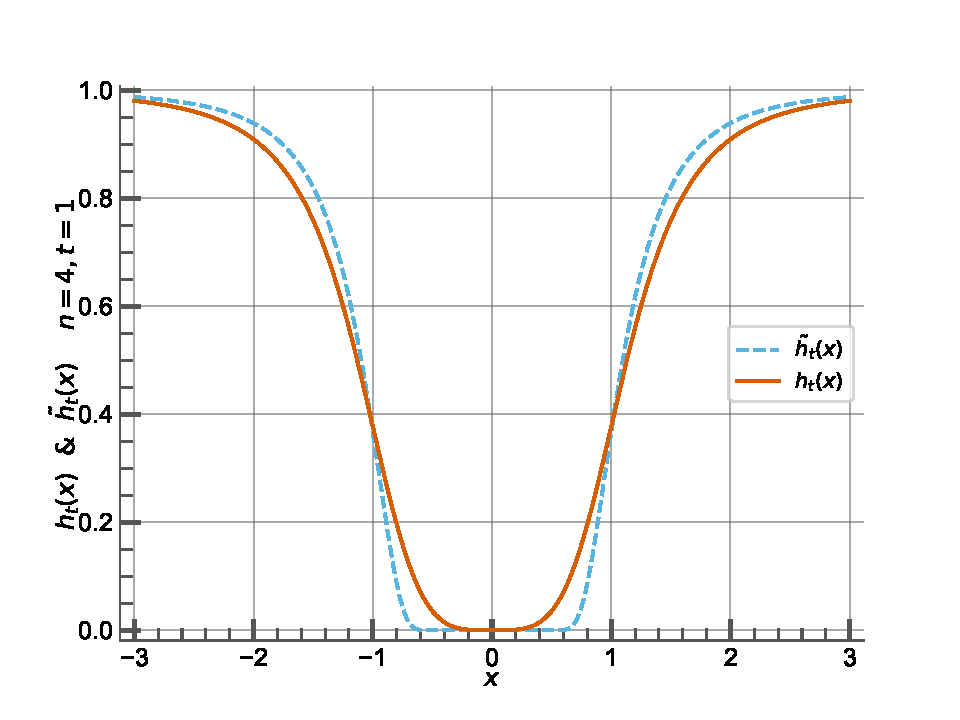
\includegraphics[width=0.5\linewidth]{chapter_1/assets/h_stable_vs_unstable.pdf}}
  \caption{\centering The unstable reparametrization function $h_t^*$ and its
  stable alternative $h_t$, with $t=1$ and $n=4$ for both functions.} 
  \label{fig:chap1:h_stable_vs_unstable}
\end{figure}

\subsection{Budget Loss}
\label{sec:chap1:budget_loss}

\section{Experiments And Results}